\chapter{Implementasi dan Pengujian Sistem HILS}\label{chapter-4}

\section{Implementasi Sistem HILS}

Berdasarkan analisis dan rancangan solusi pada Bab \ref{chapter-3}, dapat
dimulai implementasi sistem HILS baru. Implementasi sistem HILS dimulai dengan
eksplorasi ROS2 dan ZeroMQ. Kemudian dilanjutkan dengan pembuatan program
\textit{proof of concept} (POC) menggunakan salah satu mekanisme komunikasi.
POC dibuat untuk menunjukan bahwa mekanisme komunikasi yang digunakan dapat
melakukan transfer data kamera sehingga CARLA berjalan dengan setidaknya 2 FPS.
Setelah POC diterima oleh ketua tim simulasi, dilanjutkan penulisan pustaka
\textit{consumer} dan terakihir implementasi pustaka \textit{producer}.

Dari proses eksplorasi dan implementasi POC, didapatkan metode komunikasi yang
cocok adalah ZeroMQ. ROS 2 sendiri gagal pada tahap POC dikarenakan sistem
operasi tidak kompatibel dengan ROS 2. Oleh karena itu, implementasi pustaka
akan menggunakan ZeroMQ. Sedangkan, ROS 2 tidak akan digunakan lagi pada tugas
akhir ini.

Pustaka yang pertama ditulis adalah pustaka \textit{consumer} (sisi
komputer AGX/RKB) karena program utama komputer SILS (pengguna
\textit{producer}) belum selesai pada saat proses penulisan pustaka. Akibatnya,
pengujian pustaka \textit{consumer} lebih mudah dilakukan pada saat itu.

Pustaka \textit{producer} dan \textit{consumer} akan memanfaatkan pemrograman
berorientasi objek untuk menstruktur kodenya. Pustaka yang dibuat juga dibuat
seabstrak mungkin dan tidak \textit{coupled} pada trem saja. Sehingga pustaka
yang ditulis dapat digunakan untuk simulasi \textit{hardware-in-the-loop} jenis
kendaraan otonom lainnya.

Diagram kelas dari pustaka \textit{consumer} dapat dilihat pada gambar
\ref{chapter-4-consumer-class-diagram}. Kelas yang melakukan komunikasi adalah
kelas abstrak \texttt{Endpoint}. Kelas tersebut dibuat abstrak dan diinstansiasi
menggunakan pola pemrograman \textit{factory}. \texttt{Endpoint} dibuat abstrak
agar apabila ingin ditambahkan metode komunikasi lain, hal tersebut dapat
dilakukan dengan mudah. Contoh kasus penggunaan penambahan metode komunikasi
lain adalah pengujian atau \textit{benchmarking} metode komunikasi. Selain itu,
terdapat kelas yang akan menyediakan layanan untuk program GRS, yaitu
\texttt{CarlaService}. Kelas ini mengabstraksi komunikasi dan deserialisasi
ataupun serialisasi data dari \texttt{Endpoint}.
\begin{figure}[!htbp]
	\centering
	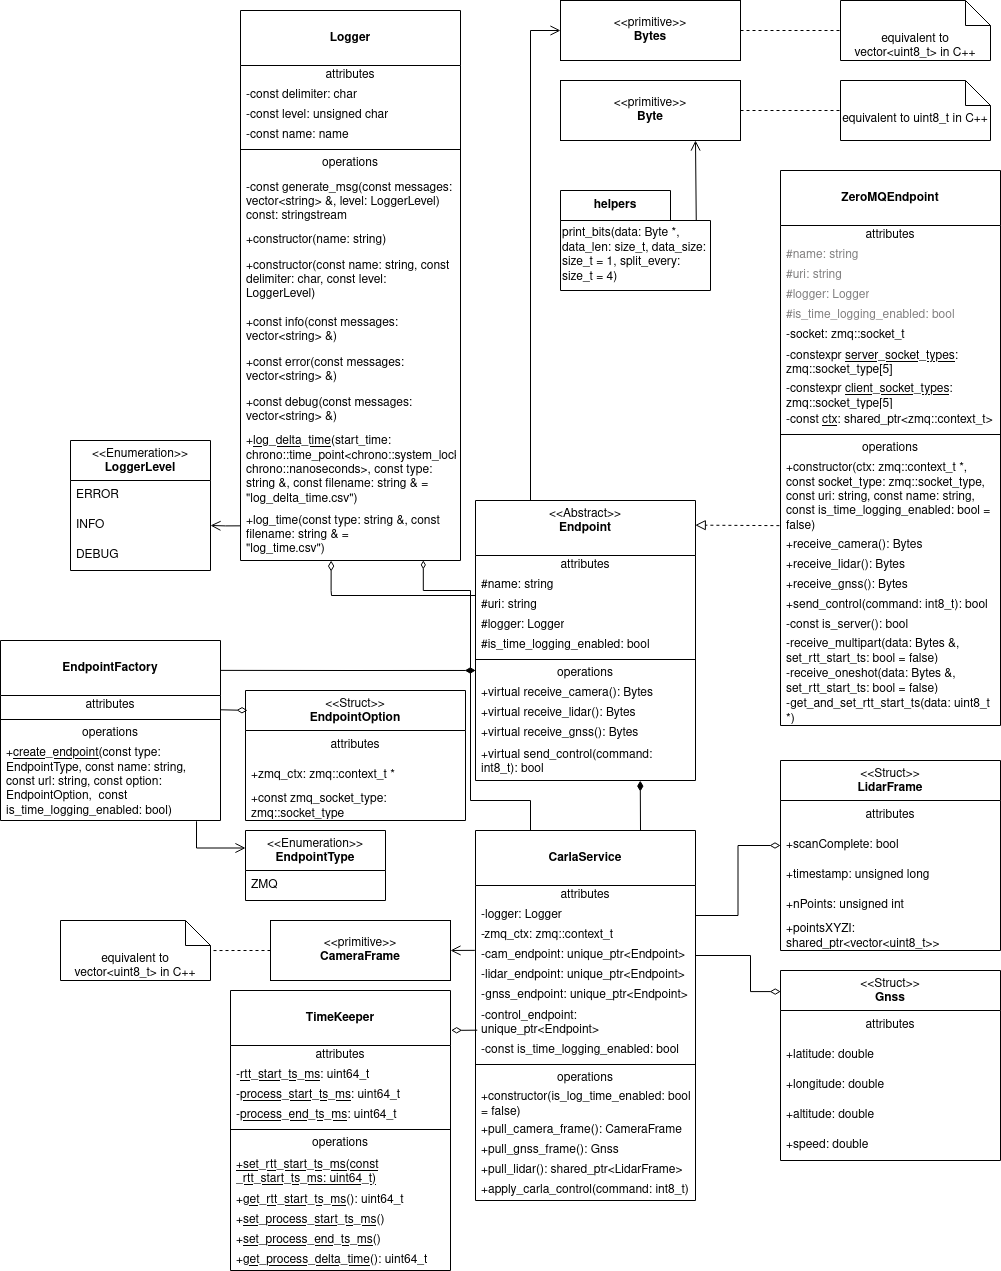
\includegraphics[width=1.0\textwidth]{resources/chapter-4/consumer-class_diagram.png}
	\caption{Diagram Kelas Pustaka \textit{Consumer}}
	\label{chapter-4-consumer-class-diagram}
\end{figure}

Setelah pustaka \textit{consumer} berhasil, implementasi dilanjutkan dengan
pembuatan pustaka \textit{producer}. Diagram kelas pustaka \textit{producer}
dapat dilihat pada gambar \ref{chapter-4-producer-class-diagram}. Pembuatan
pustaka \textit{producer} juga mengikuti filosofi penulisan pustaka
\textit{consumer}. Pustaka dibuat seabstrak mungkin sehingga tidak
\textit{coupled} dengan trem. Kelas \texttt{Endpoint} juga dibuat abstrak agar
dapat ditambahkan metode komunikasi yang lain. Perbedaan implementasi adalah
pada kelas yang berinteraksi dengan program utama. Pada pustaka
\textit{producer}, ada empat kelas yang berinteraksi dengan program utama, yaitu
\texttt{CameraHandler}, \texttt{LidarHandler}, \texttt{GnssHandler}, dan
\texttt{ControlHandler}. Keempat kelas memiliki peran masing-masing dan
terspesialisasi untuk menangani data dari sensor virtual CARLA tertentu.
\begin{figure}[!htbp]
	\centering
	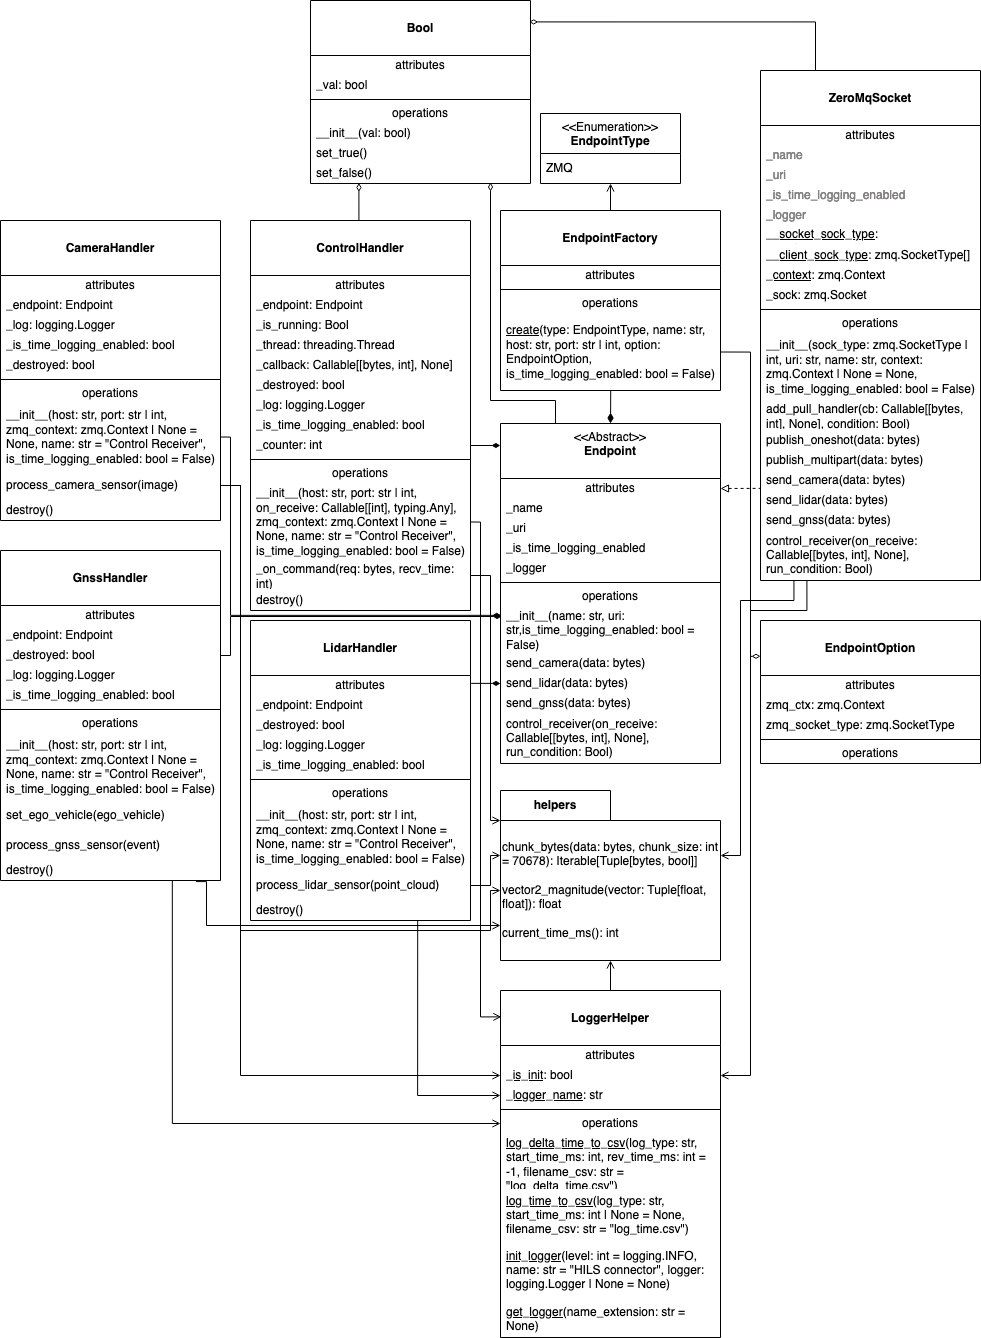
\includegraphics[width=1.0\textwidth]{resources/chapter-4/producer-class_diagram.png}
	\caption{Diagram Kelas Pustaka \textit{Producer}}
	\label{chapter-4-producer-class-diagram}
\end{figure}

Setelah kedua pustaka diimplementasi, dilakukan pengujian pustaka dengan program
kecil. Lalu, kedua pustaka diintegrasi dengan kedua program utama. Setelah itu,
dapat dianggap sistem implementasi HILS yang baru sudah diimplementasi dan
pengujian HILS dapat dilakukan. Akan tetapi untuk kebutuhan tugas akhir, sebelum
pengujian HILS dilakukan, akan dilaksanakan pengujian. Metode pengujian dan
aspek sistem yang diuji akan dibahas pada Subbab
\ref{chapter-4-testing-methodology}.

\section{Metode Pengujian Implementasi dan
  Kinerja}\label{chapter-4-testing-methodology}

Pengujian akan menguji dua aspek, yaitu
\begin{enumerate}
	\item pengujian implementasi: meninjau kemampuan sistem HILS dalam mengirim,
	      menerima, dan menggunakan data dari sensor virtual untuk
	      mengendalikan trem; dan
	\item pengujian kinerja: meninjau latensi yang dibutuhkan untuk mengirim
	      data dan meninjau kecepatan simulator saat simulasi.
\end{enumerate}
Subbab \ref{chapter-4-testing-methodology}, akan membahas metode dan rencana
pengujian kedua aspek tersebut. Selain itu, akan dibahas juga lingkungan
pengujian. Pengujian dilakukan dengan menjalankan beberapa skenario simulasi
lalu dibandingkan dengan kriteria kedua aspek. Sebuah aspek dinyatakan berhasil
apabila semua kriterianya berhasil dicapai.

\subsection{Lingkungan Pengujian}

Pengujian sistem HILS dilakukan pada laboratorium sistem kendali di Lab
Teknologi VIII ITB. Komputer yang akan digunakan pada lab tersebut ada tiga,
yaitu komputer AGX, komputer RKB, dan komputer SILS. Komputer AGX adalah NVIDIA
Drive PX Pegasus. Spesifikasi komputer AGX dapat dilihat pada Subbab
\ref{chapter-2-section-pegasus}. Sedangkan spesifikasi komputer SILS dan RKB
adalah sebagai berikut (Tabel \ref{chapter-4-tbl-environment-specs}).

\begin{table}[!htbp]
	\centering
	\begin{tabular}{|r|l|l|}
		\hline
		              & CPU & i9-10920X 12C/24T 3.50GHz  \\
		\cline{2-3}
		\textbf{SILS} & RAM & 128GB                      \\
		\cline{2-3}
		              & GPU & 2x NVIDIA GeForce RTX 3090 \\
		\cline{2-3}
		              & OS  & Ubuntu Linux 20.04         \\
		\hline
		              & CPU & i7-8700 6C/12T 3.20GHz     \\
		\cline{2-3}
		\textbf{RKB}  & RAM & 16GB                       \\
		\cline{2-3}
		              & GPU & NVIDIA GeForce RTX 2070    \\
		\cline{2-3}
		              & OS  & Ubuntu Linux 18.04         \\
		\hline
	\end{tabular}
	\label{chapter-4-tbl-environment-specs}
	\caption{Spesifikasi komputer SILS dan komputer RKB.}
\end{table}

Untuk pengujian implementasi, akan dilakukan pada komputer AGX dan komputer
SILS. Komputer AGX akan menjalankan program GRS dan komputer SILS akan
menjalankan program ScenarioRunner. Sedangkan pada pengujian kinerja komputer
yang akan digunakan adalah komputer RKB. Komputer RKB akan menggantikan fungsi
komputer AGX.

Pada pengujian kinerja, kedua komputer (komputer RKB dan komputer SILS)
terhubung pada sebuah jaringan lokal (LAN). Topologi jaringan dapat dilihat di
Gambar \ref{chapter-4-fig-topology}. Komputer SILS dan komputer RKB terhubung
melalu sebuah \textit{switch} HPE JH019A. Komputer SILS terhubung ke
\textit{switch} menggunakan sebuah cabel Cat5. Sedangkan komputer RKB terhubung
ke \textit{switch} menggunakan sebuah cabel Cat6 bermerk Commscope 1071E.

\begin{figure}[!htbp]
	\centering
	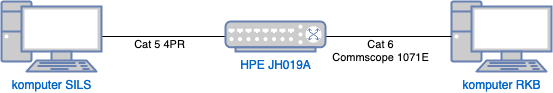
\includegraphics[width=1.0\textwidth]{resources/chapter-4/test-environment-network-topology.png}
	\caption{Topologi lingkungan pengujian}
	\label{chapter-4-fig-topology}
\end{figure}

\subsection{Pengujian Implementasi Sistem HILS}

Pengujian implementasi dilakukan dengan menjalankan program utama di komputer
SILS dan komputer AGX/RKB. Kemudian, akan dilakukan observasi untuk memeriksa
sistem HILS sudah memenuhi kriteria-kriteria pada Tabel
\ref{chapter-4-tbl-impl-criteria} atau belum.

\begin{table}[!htbp]
	\begin{center}
		\begin{tabular}{|l|l|}
			\hline
			\textbf{Kode} & \textbf{Deskripsi}                                     \\
			\hline
			IMPL-01       & Kecepatan trem di program GRS sesuai dengan bacaan
			sensor                                                                 \\
			              & GNSS.                                                  \\
			\hline
			IMPL-02       & Tampilan kamera di program GRS sesuai dengan yang
			ada di                                                                 \\
			              & program ScenarioRunner.                                \\
			\hline
			IMPL-03       & Tampilan lidar di program GRS menampikan
			objek-objek                                                            \\
			              & yang ada di sekitar trem.                              \\
			\hline
			IMPL-04       & Trem maju ketika mendapatkan kendali maju dan berhenti \\
			              & ketika mendapatkan kendali berhenti.                   \\
			\hline
		\end{tabular}
	\end{center}

	\caption{Kriteria pengujian implementasi sistem HILS}
	\label{chapter-4-tbl-impl-criteria}
\end{table}

Kriteria ini selaras dengan tujuan tugas akhir yang kedua, yaitu
mengimplementasikan sistem simulasi yang dapat mengirimkan, menerima, dan
memanfaatkan data dari berbagai jenis sensor.

\subsection{Pengujian Kinerja Sistem HILS}

Dari segi kinerja, hal yang ingin dipastikan adalah CARLA dapat berjalan stabil
dengan kecepatan minimum 2 FPS (\textit{frames per second}). Hal tersebut
diobservasi dengan menjalankan kedua program utama. Selain dari kecepatan
simulator, aspek kinerja juga akan dinilai dari perbandingan dengan sistem HILS
yang ada. Latensi pengiriman data harus lebih rendah dibandingkan latensi sistem
HILS yang ada. Kedua kriteria tersebut dituangkan pada Tabel
\ref{chapter-4-tbl-perf-criteria}.
\begin{table}[!htbp]
	\begin{center}
		\begin{tabular}{|l|l|}
			\hline
			\textbf{Kode} & \textbf{Deskripsi}                                       \\
			\hline
			              & CARLA dapat berjalan dengan stabil dengan kecepatan      \\
			PERF-01       & minimum 2 FPS ketika simulasi menggunakan sensor         \\
			              & kamera dan GNSS.                                         \\
			\hline
			PERF-02       & Latensi pengiriman data lebih rendah dibandingkan sistem \\
			              & HILS yang ada.                                           \\
			\hline
		\end{tabular}
	\end{center}
	\caption{Kriteria pengujian kinerja sistem HILS}
	\label{chapter-4-tbl-perf-criteria}
\end{table}

Pengujian kriteria PERF-02 akan menggunakan \textit{round-trip time} (RTT) yang
dibagi dua untuk perkiraan latensi sistem. Rumus perhitungan RTT dapat dilihat
pada persamaan \ref{chapter-4-eq-rtt}.
\begin{equation}
	\label{chapter-4-eq-rtt}
	\text{RTT} = T_{e} - T_{s} - t_p
\end{equation}

Dengan keterangan persamaan sebagai berikut.
\begin{table}[!h]
	\begin{tabular}{l l}
		RTT     & :     \textit{round-trip time} (dalam ms)             \\
		$T_{e}$ & : \textit{timestamp} didapatkan kendali (dalam ms)    \\
		$T_{s}$ & : \textit{timestamp} dikirimkan segmen pertama kamera
		(dalam ms)                                                      \\
		$t_p$   & :   waktu pemrosesan (dalam ms)
	\end{tabular}
\end{table}

Untuk perhitungan RTT digunakan sensor kamera karena sensor kamera memiliki
ukuran terbesar sehingga diharapkan dapat menjadi kasus terburuk untuk mekanisme
komunikasi. Lalu, karena data kamera ukurannya besar, maka pengiriman data
kamera harus dibagi menjadi beberapa segmen. Karena ada beberapa segmen,
perhitungan RTT dilakukan dari segmen pertama agar latensi yang dihitung adalah
latensi keseluruhan pengiriman data kamera, tidak hanya sebuah segmen.

Pada implementasi tugas akhir ini, perhitungan RTT ($T_s$) sendiri dimulai
sebelum pemanggilan fungsi ZeroMQ untuk melakukan pengiriman segmen pertama.
Sedangkan $T_e$ dihitung dari waktu pertama kali data kendali diterima. Karena
perhitungan dimulai sebelum data kamera dikirim dan setelah data kendali
diterima, artinya RTT dihitung pada sisi program ScenarioRunner (komputer SILS).
Sedangkan $t_p$ adalah total waktu yang dibutuhkan sejak data pertama kamera diterima
sampai kendali siap dikirimkan (sebelum pemanggilan fungsi ZeroMQ).

Selain itu, pada pengujian pengujian kriteria PERF-02 untuk implementasi HILS
sebelumnya akan dilakukan secara teoretis. Hal ini karena implementasi HILS
sebelumnya sudah sulit untuk dijalankan. Selain itu, jenis data yang dikirim
pada implementasi HILS sebelumnya juga berbeda. Pengujian secara teoretis ini
dilakukan dengan menulis ulang sebagian dari mekanisme komunikasi implementasi
HILS sebelumnya. Bagian yang akan ditulis ulang adalah operasi pembacaan data
dari \textit{file}, penulisan dan pembacaan ke basis data, serta penulisan data
sensor yang dibaca dari basis data ke \textit{file}. Dengan demikian, ada 4
operasi I/O dari implementasi HILS sebelumnya yang ditulis ulang untuk pengujian
latensi secara teoretis.

Apabila sistem HILS berhasil memenuhi kedua kriteria tersebut, sistem dapat
dianggap sudah berhasil memenuhi tujuan pertama tugas akhir. Tujuan yang
dipenuhi adalah tujuan pertama tugas akhir, yaitu membuat sistem simulasi
\textit{hardware-in-the-loop} yang cukup cepat.

Pengujian kinerja sistem HILS baru akan menggunakan komputer RKB dan komputer
SILS. Komputer RKB akan menjalankan program GRS dan komputer SILS akan
menjalankan simulator CARLA serta program ScenarioRunner. Lalu, pengujian sistem
HILS lama akan menggunakan komputer SILS saja. Artinya, pada implementasi ulang
sistem HILS lama, tidak akan ada komunikasi antar-komputer dan semua proses
terjadi secara lokal.

\section{Hasil Pengujian}

Penjabaran hasil pengujian aspek implementasi dan kinerja akan dipisah.
Penjabaran dipisah karena hal yang diujikan serta kriteria pengujian dari kedua
aspek berbeda.

\subsection{Hasil Pengujian Implementasi Sistem HILS}

Dari pengujian yang dilakukan, ditemukan bahwa sistem HILS dapat memenuhi
seluruh kriteria yang untuk pengujian implementasi sistem. Penjabaran
ketercapaian kriteria pengujian implementasi sistem HILS dapat dilihat pada
\ref{chapter-4-tbl-impl-criteria-result}. Selain itu, tampilan sistem HILS dan
hasil implementasi dapat dilihat pada gambar \ref{chapter-4-fig-hils-running}.

Pada gambar \ref{chapter-4-fig-hils-running}, dapat dilihat sistem simulasi
sudah dijalankan di komputer AGX dan komputer SILS. Komputer SILS ditampilkan di
komputer sebelah kiri menggunakan bantuan program AnyDesk. Seperti yang
terlihat, sistem simulasi sudah berjalan dengan baik. Tampilan kamera di program
ScenarioRunner (SILS) dan program GRS (AGX) sudah sama.

\begin{table}[!htbp]
	\begin{center}
		\begin{tabular}{|l|l|l|}
			\hline
			\textbf{Kode} & \textbf{Deskripsi}                         & \textbf{Tercapai} \\
			\hline
			              & Kecepatan yang ditampilkan GUI pada        &                   \\
			IMPL-01       & program ScenarioRunner dan pada program    & \checkmark        \\
			              & GRS sudah sama.                            &                   \\
			\hline
			IMPL-02       & Frame kamera yang tampil pada GUI program  & \checkmark        \\
			              & ScenarioRunner dan program GRS sudah sama. &                   \\
			\hline
			IMPL-03       & Data dari lidar sudah menampilkan objek    & \checkmark        \\
			              & sekitar trem di GUI program GRS.           &                   \\
			\hline
			              & Trem di CARLA sudah dapat bergerak tanpa   &                   \\
			IMPL-04       & butuh masukan di program ScenarioRunner    & \checkmark        \\
			              & dan sesuai dengan luaran kendali dari      &                   \\
			              & program GRS.                               &                   \\
			\hline
		\end{tabular}
	\end{center}

	\caption{Tercapainya pengujian implementasi atau tidak.}
	\label{chapter-4-tbl-impl-criteria-result}
\end{table}

\begin{figure}[!htbp]
	\centering
	\includegraphics[width=1.0\textwidth,trim={12cm 12cm 0 12cm},clip]{resources/chapter-4/HILS-system-running.png}
	\caption{Tampilan sistem HILS ketika dijalankan. Tampilan komputer SILS di
		sebelah kiri, tampilan komputer AGX di sebelah kanan.}
	\label{chapter-4-fig-hils-running}
\end{figure}

\subsection{Hasil Pengujian Kinerja Sistem HILS}

Hasil pengujian kinerja sistem HILS dapat dilihat pada Tabel \ref{chapter-4-tbl-perf-criteria-result}.
\begin{table}[!htbp]
	\begin{center}
		\begin{tabular}{|l|l|l|}
			\hline
			\textbf{Kode} & \textbf{Deskripsi}                              & \textbf{Tercapai} \\
			\hline
			              & Sistem HILS berhasil memiliki kinerja yang baik &                   \\
			              & ketika hanya sensor kamera dan GNSS yang        &                   \\
			PERF-01       & digunakan. CARLA berhasil mendapatkan lebih     & \checkmark$^*$    \\
			              & dari 10 FPS. Akan tetapi, apabila ada sensor    &                   \\
			              & lidar CARLA gagal mencapai 2 FPS.               &                   \\
			\hline
			PERF-02       & Sistem HILS baru berhasil memiliki kinerja yang & \checkmark        \\
			              & lebih baik daripada sistem HILS sebelumnya.     &                   \\
			\hline
		\end{tabular}
	\end{center}

	\caption{Tercapainya pengujian implementasi atau tidak.}
	\label{chapter-4-tbl-perf-criteria-result}
\end{table}

Kriteria PERF-01 berhasil dipenuhi karena ketika menggunakan sensor kamera dan
GNSS kinerja sistem sangat baik. Akan tetapi, jika duji dengan sensor lidar
sistem HILS tidak memiliki kinerja yang baik. Simulator CARLA gagal mendapatkan
2 FPS. Kendati demikian, PERF-01 dapat dianggap berhasil karena pengujian cukup
dengan sensor kamera dan  sensor GNSS.

Kriteria PERF-02 juga berhasil dilewati. Dapat dilihat pada Tabel
\ref{chapter-4-tbl-perf-result-statistics}, implementasi HILS baru memiliki
latensi setidaknya 2,5 kali lebih cepat dari implementasi teoretis HILS
sebelumnya. Selain itu, persebaran data latensi kedua implementasi sistem HILS
dapat dilihat pada Gambar \ref{chapter-4-fig-perf-result-old-hils} dan Gambar
\ref{chapter-4-fig-perf-result-new-hils}.
\begin{table}[!htbp]
	\begin{center}
		\begin{tabular}{|l|l|l|}
			\hline
			                   & Jumlah data    & 1.000     \\
			\cline{2-3}
			                   & Rata-rata (ms) & 28,4245   \\
			\cline{2-3}
			                   & Std (ms)       & 4,68      \\
			\cline{2-3}
			\textbf{HILS lama} & Min (ms)       & 16        \\
			\cline{2-3}
			(teoretis)         & $Q_1$ (ms)     & 25        \\
			\cline{2-3}
			                   & $Q_2$ (ms)     & 28        \\
			\cline{2-3}
			                   & $Q_3$ (ms)     & 31        \\
			\cline{2-3}
			                   & Max (ms)       & 45,5      \\
			\cline{2-3}
			\hline

			\hline
			                   & Jumlah data    & 16.891    \\
			\cline{2-3}
			                   & Rata-rata (ms) & 10,989965 \\
			\cline{2-3}
			                   & Std (ms)       & 2,248782  \\
			\cline{2-3}
			\textbf{HILS baru} & Min (ms)       & 4,5       \\
			\cline{2-3}
			                   & $Q_1$ (ms)     & 10        \\
			\cline{2-3}
			                   & $Q_2$ (ms)     & 11        \\
			\cline{2-3}
			                   & $Q_3$ (ms)     & 12,5      \\
			\cline{2-3}
			                   & Max (ms)       & 19,5      \\
			\cline{2-3}
			\hline
		\end{tabular}
	\end{center}

	\caption{Statistik data hasil pengujian kinerja}
	\label{chapter-4-tbl-perf-result-statistics}
\end{table}
\begin{figure}[!htbp]
	\centering
	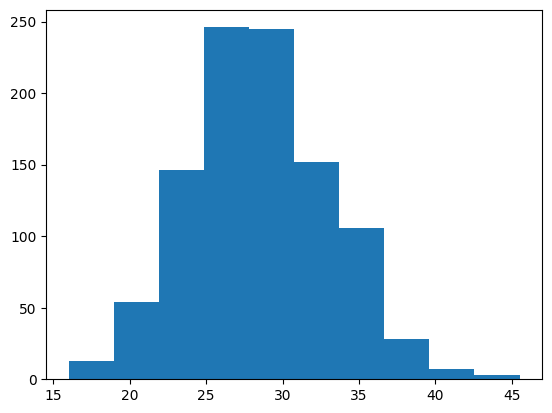
\includegraphics[width=1.0\textwidth]{resources/chapter-4/old-hils-data.png}
	\caption{Persebaran data latensi untuk implementasi teoretis HILS lama}
	\label{chapter-4-fig-perf-result-old-hils}
\end{figure}
\begin{figure}[!htbp]
	\centering
	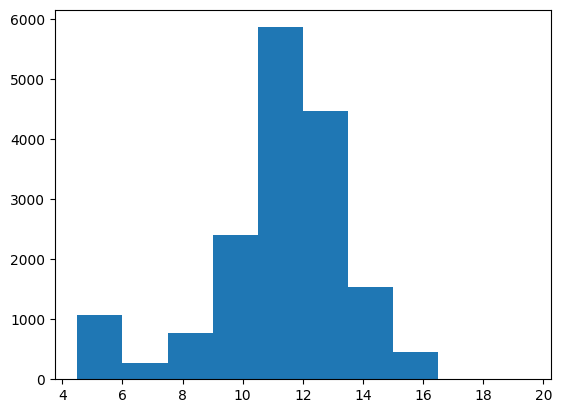
\includegraphics[width=1.0\textwidth]{resources/chapter-4/new-hils-data.png}
	\caption{Persebaran data latensi untuk implementasi HILS baru}
	\label{chapter-4-fig-perf-result-new-hils}
\end{figure}

Keberhasilan PERF-02 dikonfirmasi dari penggunaan \textit{resource} komputer
pada kedua komputer. Ketika menjalankan sistem HILS baru, penggunaan
\textit{resource}-nya dapat dilihat pada Gambar
\ref{chapter-4-fig-perf-result-resource-usage-sils} (komputer SILS) dan Gambar
\ref{chapter-4-fig-perf-result-resource-usage-rkb} (komputer RKB). Dapat dilihat
pada implementasi baru HILS, penggunaan CPU-nya belum mencapai 50\% dan
penggunaan RAM juga belum mencapai 10\%. Rata-rata penggunaan CPU berkisar dari
30\%--40\%. Akan tetapi, dapat dilihat juga pada Gambar
\ref{chapter-4-fig-perf-result-resource-usage-sils-startup} (komputer SILS) dan
Gambar \ref{chapter-4-fig-perf-result-resource-usage-rkb-startup} (komputer RKB)
bahwa ada anomali yang menyebabkan penggunaan CPU melebihi 70\%.  Hal ini
terjadi ketika kedua program baru pertama kali dijalankan.
\begin{figure}[!htbp]
	\centering
	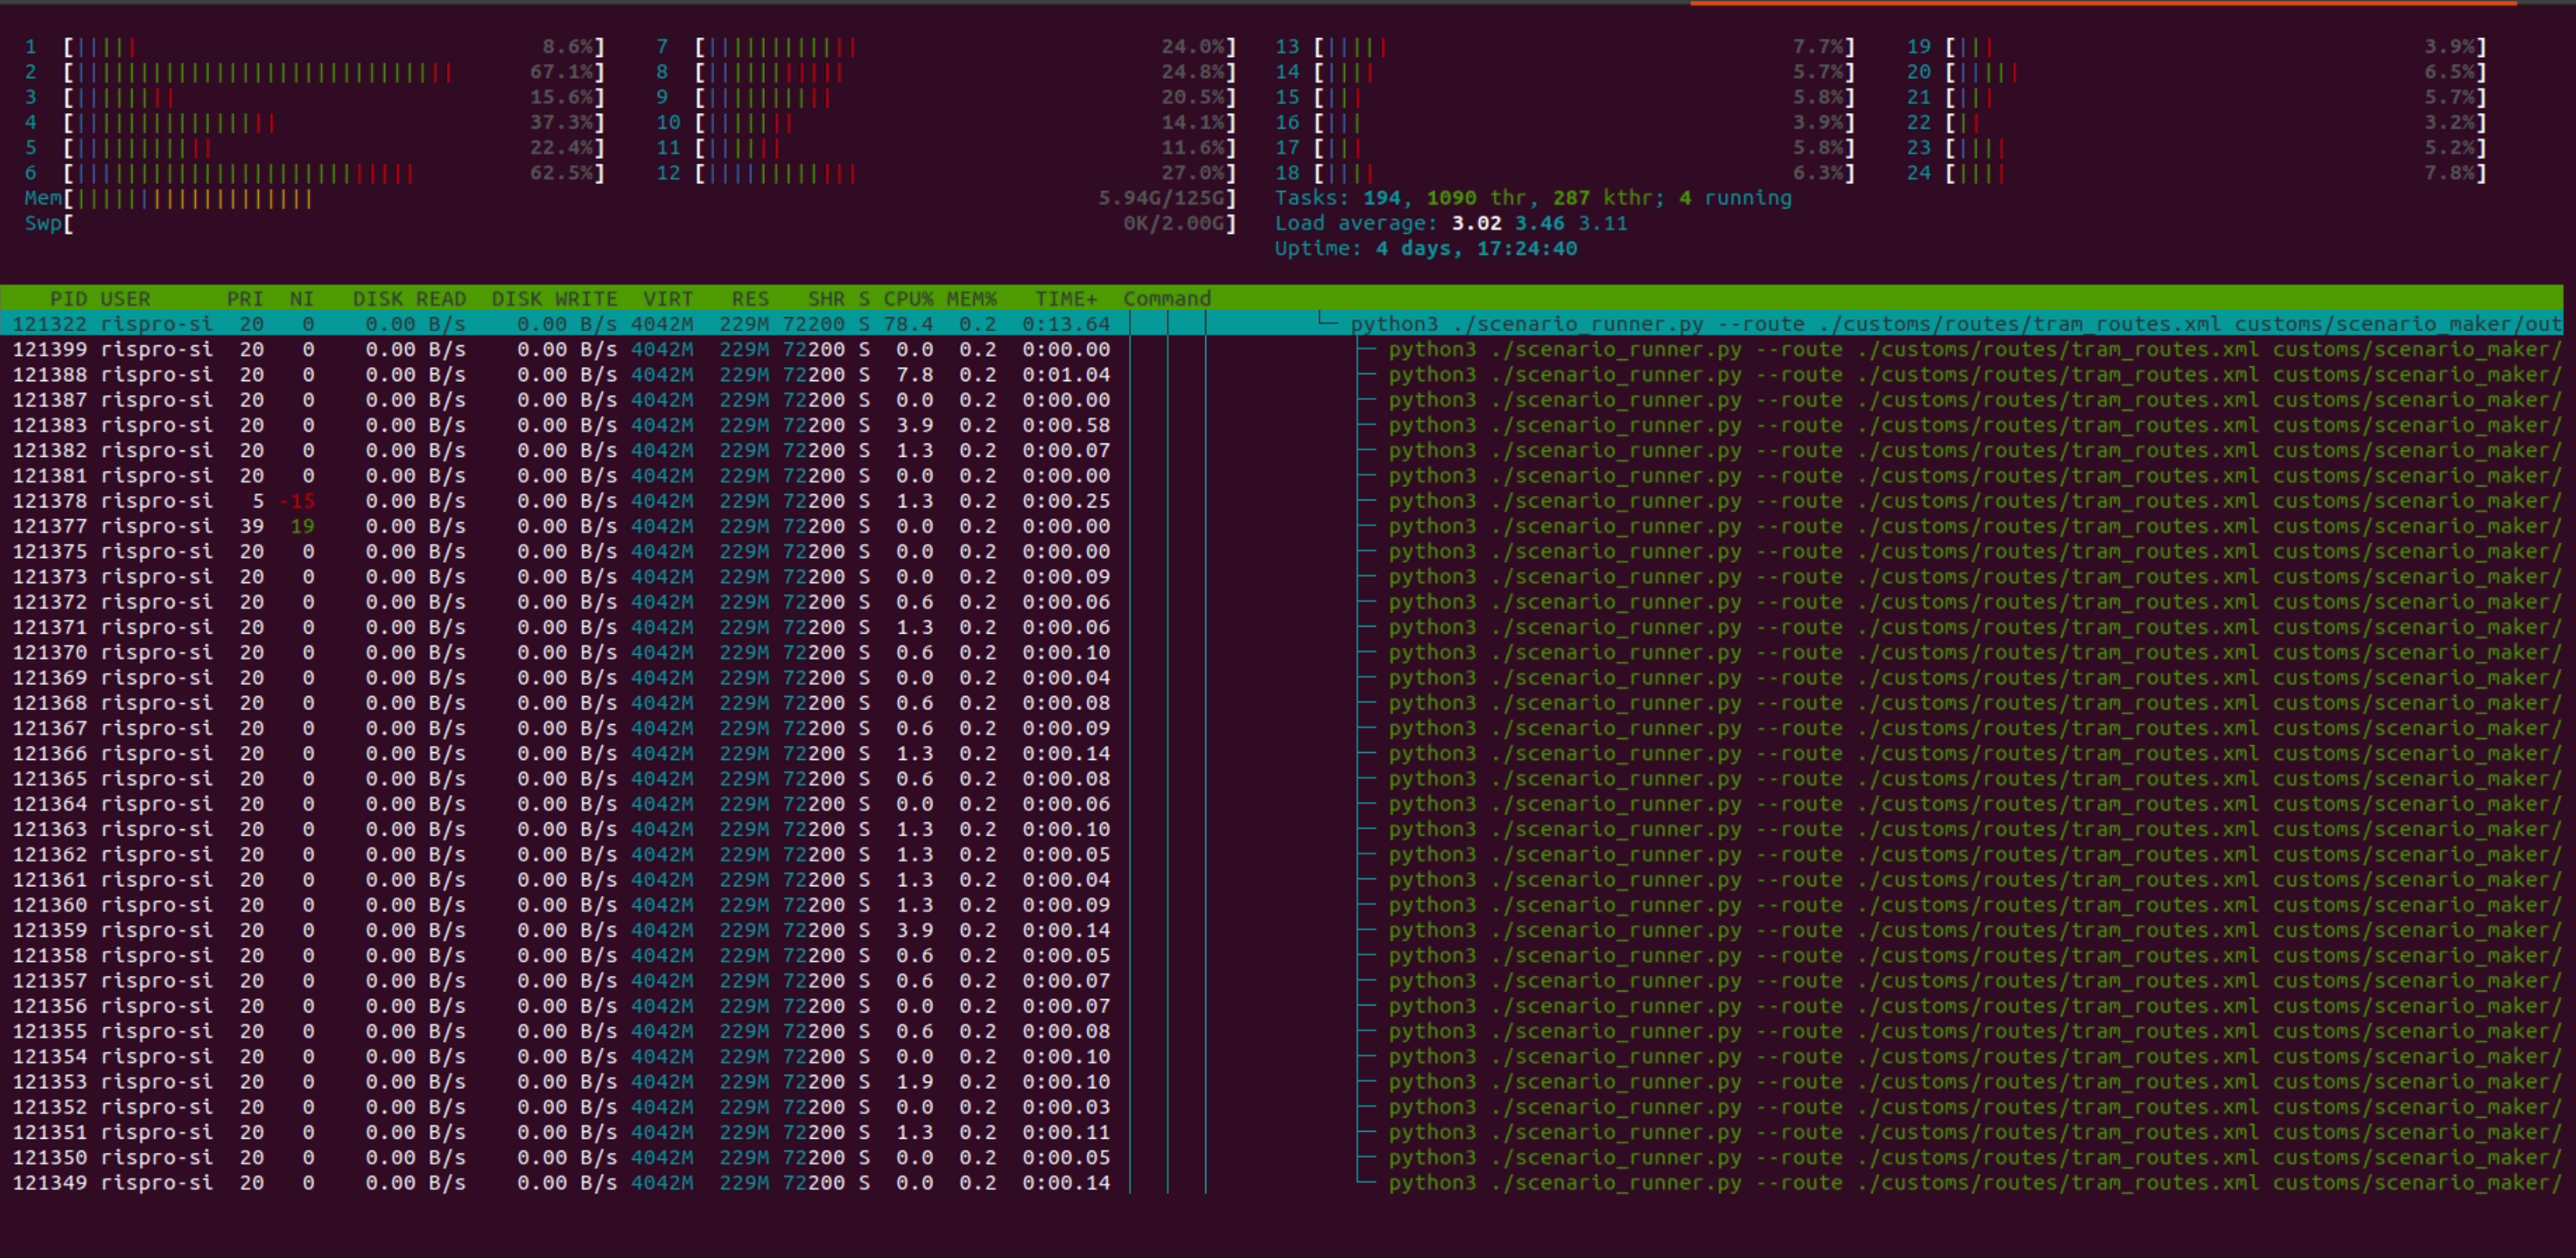
\includegraphics[width=1.0\textwidth]{resources/chapter-4/resource-usage-new-hils-sils-startup.png}
	\caption{Penggunaan \textit{resource} komputer SILS ketika menjalankan sistem HILS baru.}
	\label{chapter-4-fig-perf-result-resource-usage-sils}
\end{figure}
\begin{figure}[!htbp]
	\centering
	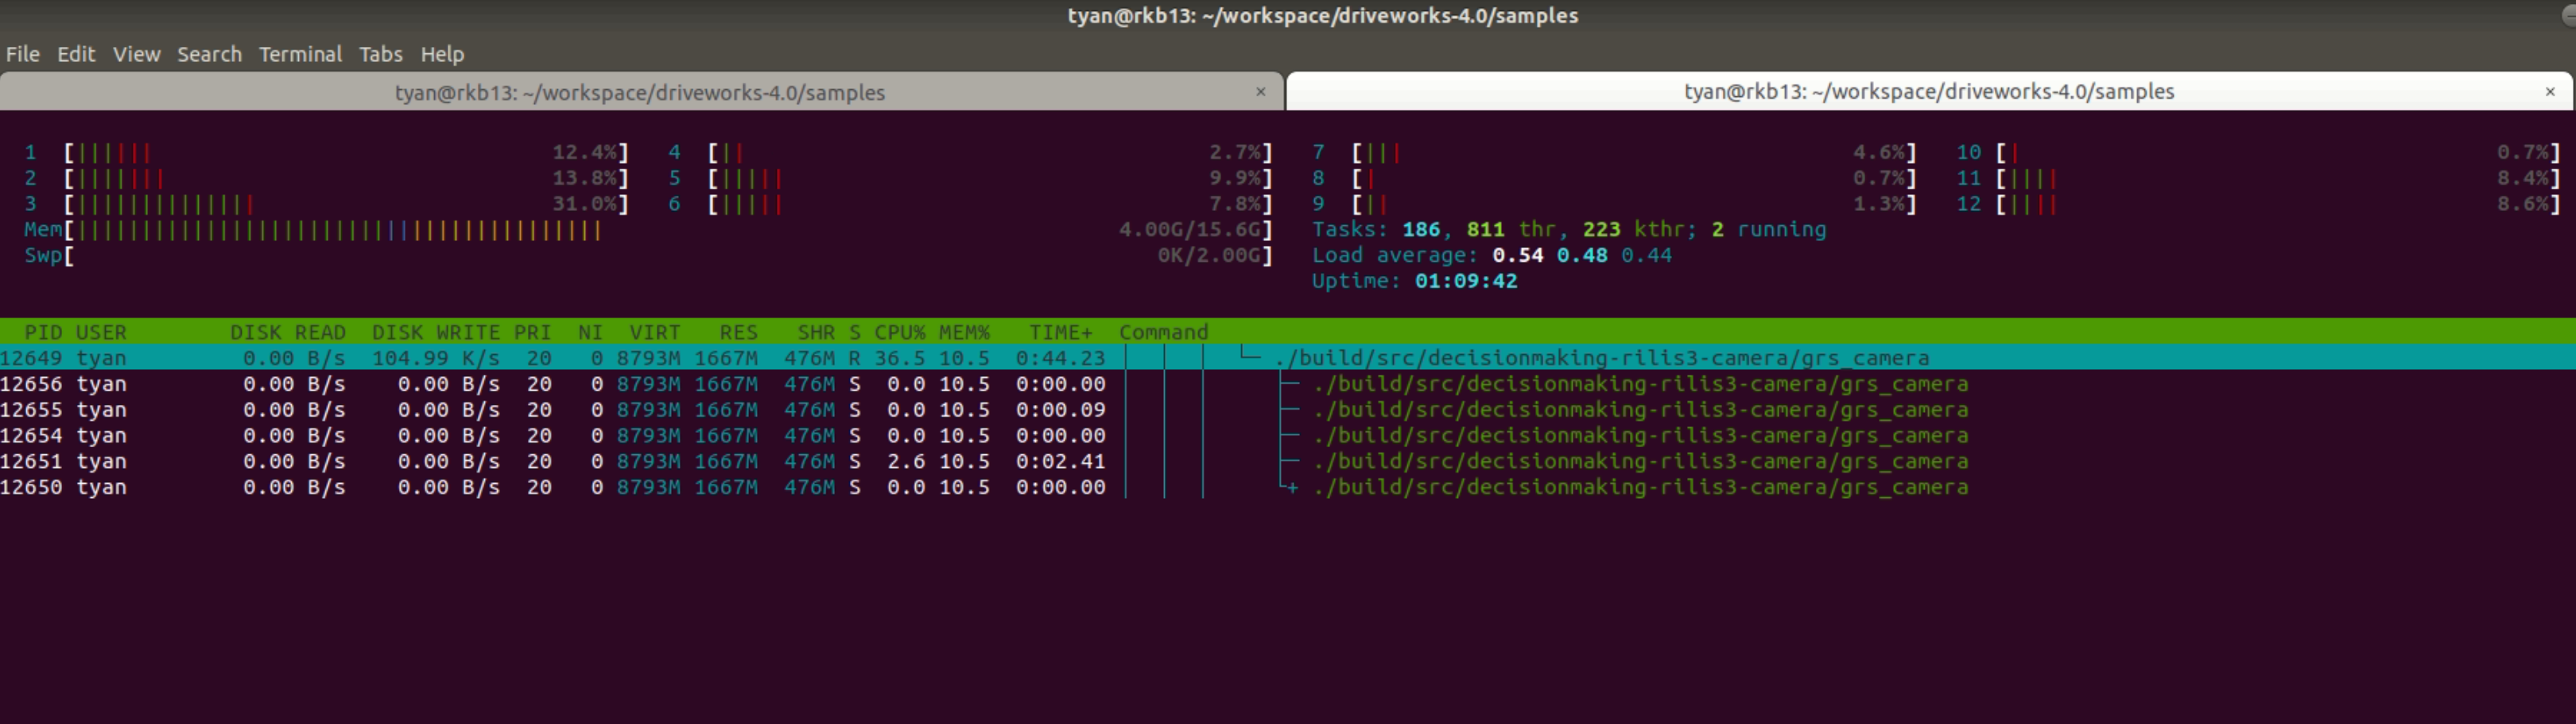
\includegraphics[width=1.0\textwidth,trim={0cm 0cm 0cm 2.5cm},clip]{resources/chapter-4/resource-usage-new-hils-rkb.png}
	\caption{Penggunaan \textit{resource} komputer SILS ketika memulai sistem HILS baru.}
	\label{chapter-4-fig-perf-result-resource-usage-sils-startup}
\end{figure}
\begin{figure}[!htbp]
	\centering
	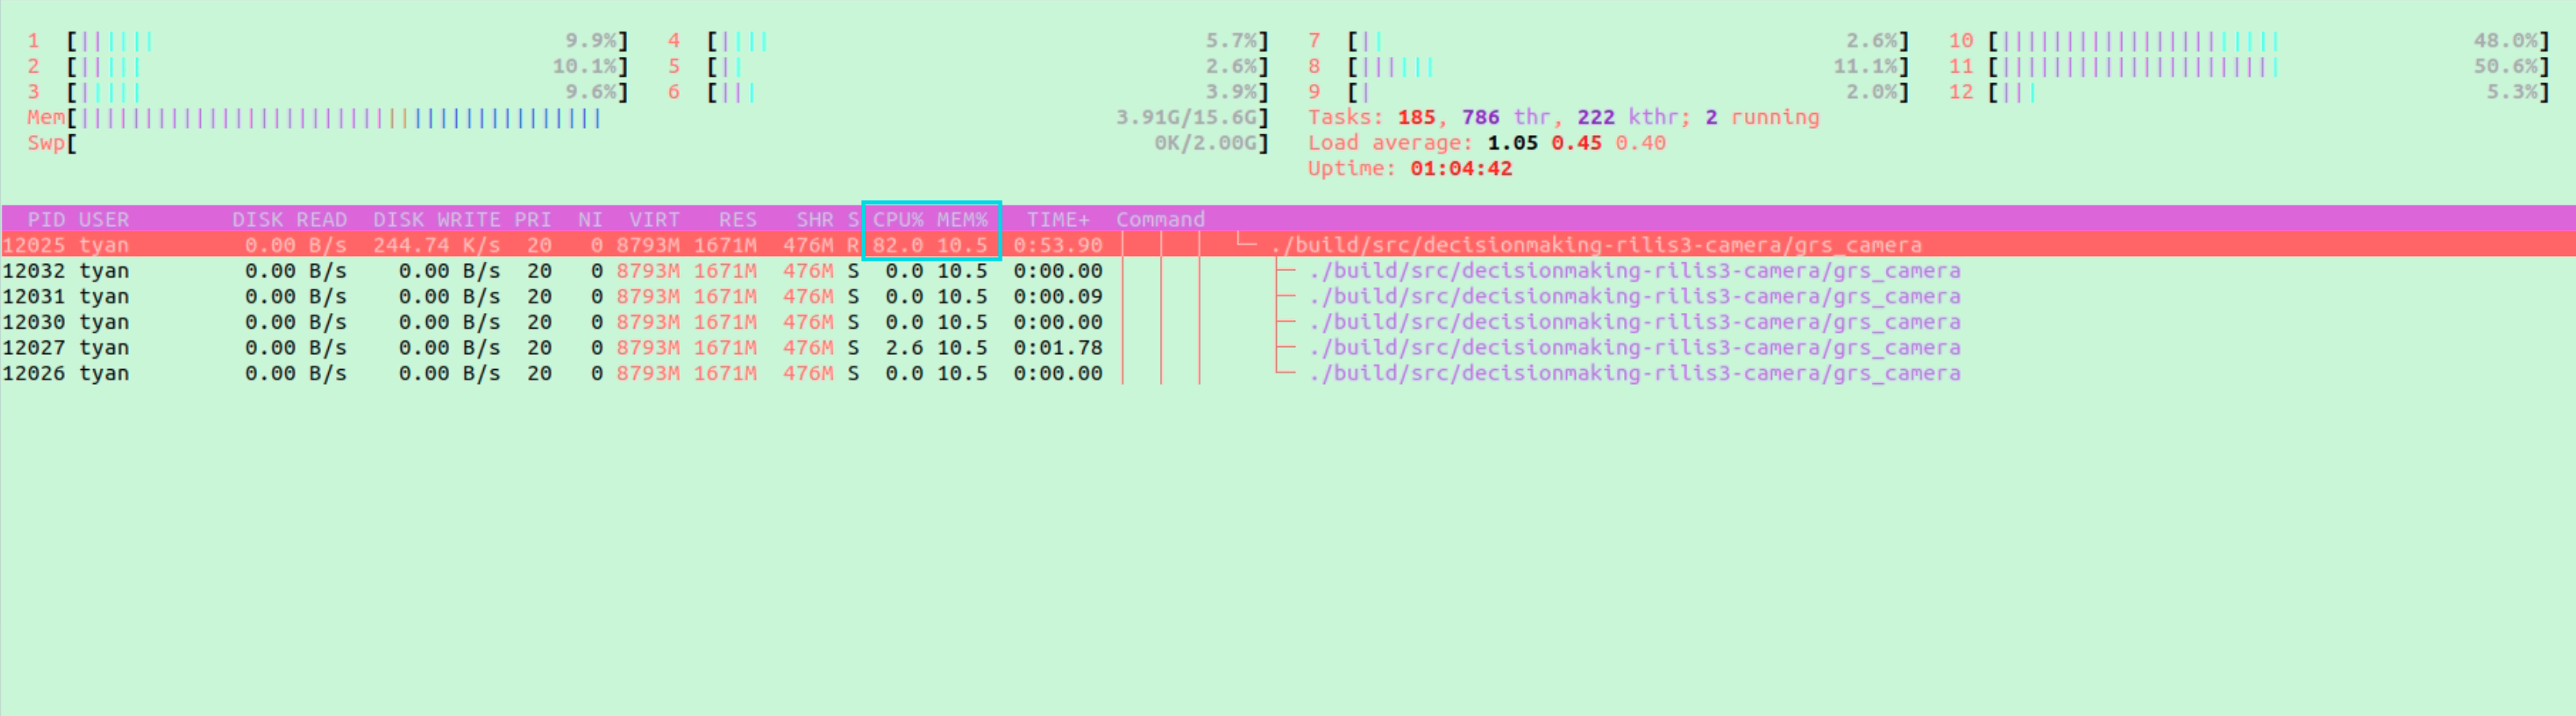
\includegraphics[width=1.0\textwidth]{resources/chapter-4/resource-usage-new-hils-rkb-startup.png}
	\caption{Penggunaan \textit{resource} komputer RKB ketika menjalankan sistem HILS baru.}
	\label{chapter-4-fig-perf-result-resource-usage-rkb}
\end{figure}
\begin{figure}[!htbp]
	\centering
	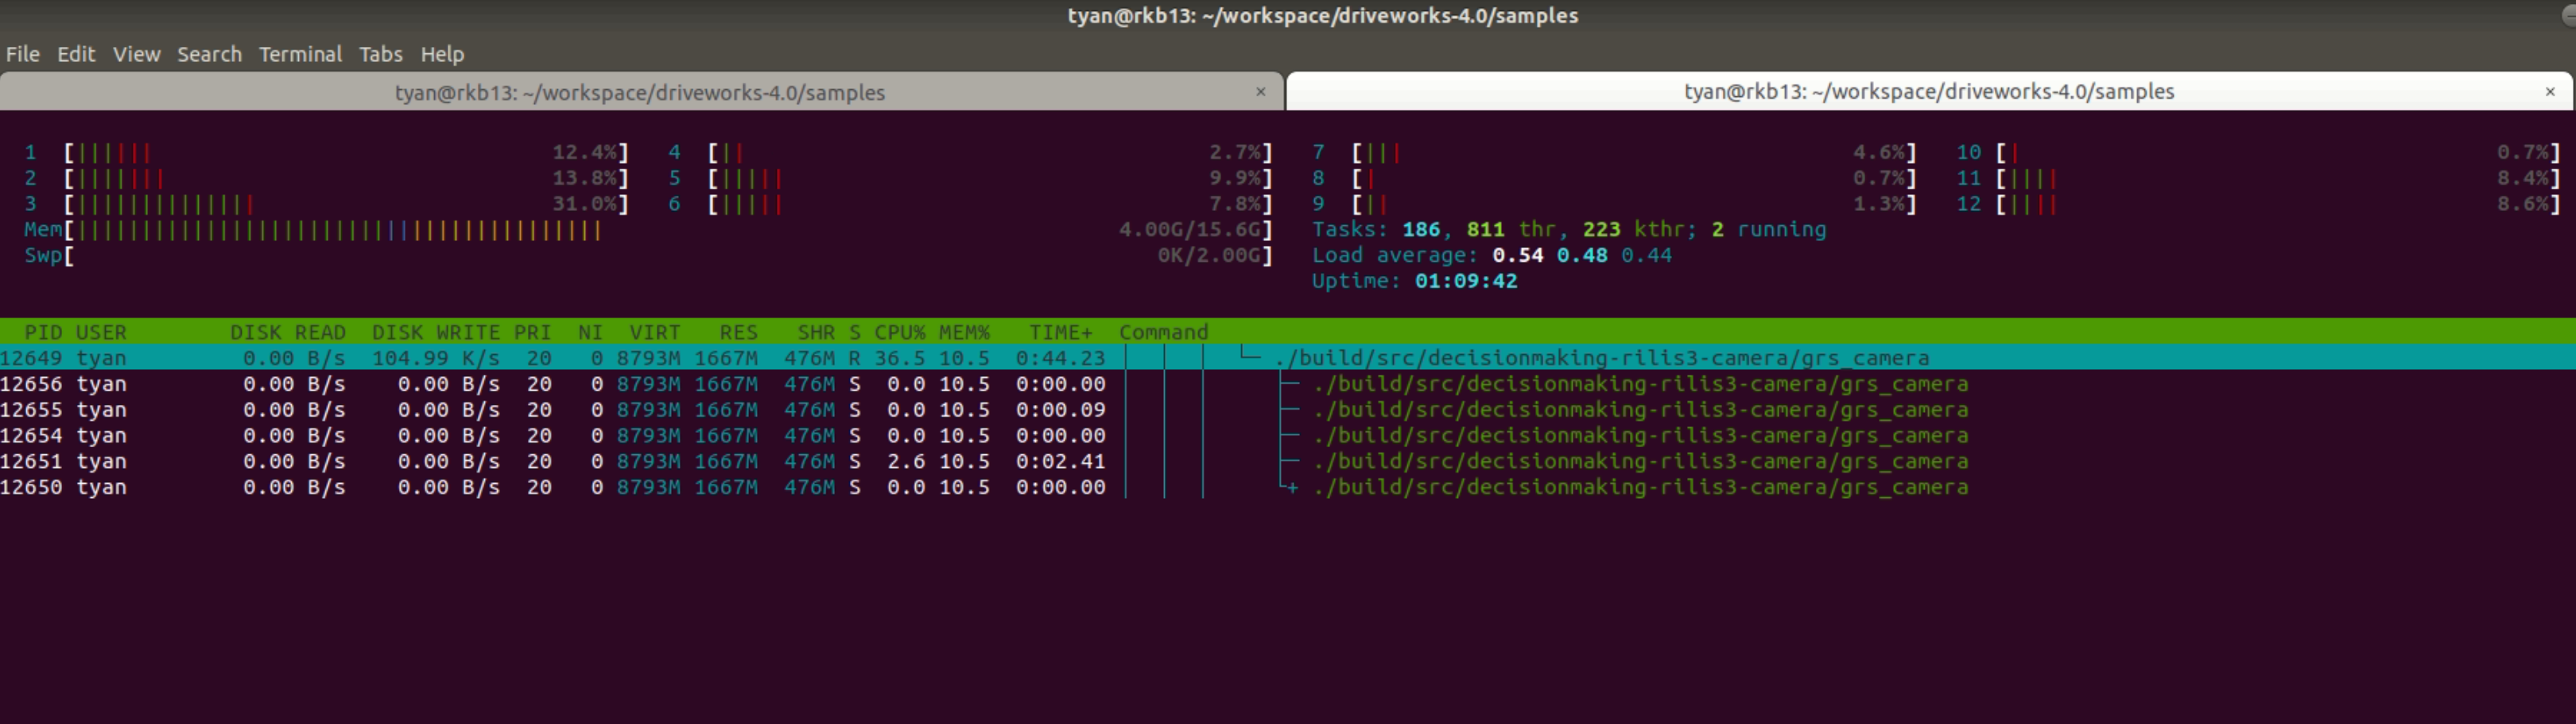
\includegraphics[width=1.0\textwidth,trim={0cm 0cm 0cm 2.5cm},clip]{resources/chapter-4/resource-usage-new-hils-rkb.png}
	\caption{Penggunaan \textit{resource} komputer RKB ketika memulai sistem HILS baru.}
	\label{chapter-4-fig-perf-result-resource-usage-rkb-startup}
\end{figure}

Data lengkap untuk menghitung RTT di pengujian kinerja dapat dilihat pada
Lampiran \ref{appendix-performance-data}. Selain itu, program Jupyter Notebook
yang digunakan untuk pemrosesan data tersebut dapat dilihat pada lampiran
\ref{appendix-algoritma-monitoring}.

\section{Pembahasan}
\blindtext
